\section{Introduction}
\label{sec:introduction}
Active public debate is vital for democracy because it can broaden access to information and public accountability. News-website forums act as modern \emph{letters to the editor}, connecting journalists and readers while exposing the difficulties of maintaining useful discussion in the presence of incivility and polarisation. News organisations also curate user-generated content, and those editorial choices need not coincide with what readers choose to endorse. Prior work describes a broader ``news gap'' between the kinds of news supplied by journalists and what attracts audience attention \citep{Boczkowski2013}; here we study an analogous gap within discussion sections attached to news articles, between comments selected by journalists and comments endorsed by readers.
Prior work has characterised professional editor-picks and their relationship to user engagement \citep{Diakopoulos2015,He2024,Wang2021}, but less is known about how editorial and audience selections align when they operate over the same discussion-specific comment set. This paper studies that comparative \emph{news comment gap}, oriented around the following three research questions:

\begin{enumerate}[label=RQ\arabic*]
\item How large is the comment gap between readers and journalists?
\item Which comment-text, discussion-context, timing, and author-history characteristics are associated with reader versus journalist selections?
\item How successfully can we predict reader and journalist selections for held-out discussions?
\end{enumerate}

The dataset contains 2.39 million comments across 5,118 articles from 2025, gathered from one of the largest German-speaking news forums hosted by the Austrian newspaper \textit{Der Standard}. Textual and contextual features of the comments are used to model “Editors’ Picks” and user votes through regression and machine learning models, thus helping us understand how journalist and reader preferences overlap and diverge.

\section{Related Work}

\subsection{News engagement}
\emph{News values} guide journalistic assessments of newsworthiness \citep{Harcup2017}, but news supply and audience demand diverge: journalists tend to prioritise public affairs while readers favour sports, entertainment, and crime \citep{Boczkowski2013}. According to Boczkowski and Mitchelstein, this ``news gap'' is substantial: journalists’ top stories had 19 percentage points more public-affairs articles than the most popular reader stories. \citet{Bright2016} explored the ``social news gap'', noting that social sharing behaviour is driven more by social status than emotion. Online news consumption and rising competition make it easier for readers to selectively engage with stories, exacerbating the news gap.

Motivations for commenting on news differ from reading and sharing, affecting the nature of any news gap. Active commenters are a specific subset: on \emph{derstandard.at} online readers are roughly gender-balanced (45\% female, 55\% male), but only 20\% of active commenters are female \citep{KrennPetrak2021}. Emotion drives engagement---anger and anxiety increase it, while positive emotions have mixed effects \citep{Diakopoulos2011, Naab2022, Ziegele2018, MarcusNeumanMacKuen2000, Berger2012}. News factors such as `controversy' and `damage' in articles also increase the likelihood of discussing and commenting on news \citep{Weber2014}. News values and discussion factors both influence the quantity and quality of comments \citep{Ziegele2018}.

News website comments differ from social media comments on news, even when they concern the same articles. Compared with social-media comments, news-site comments tend to be more deliberative, topic-focused, socially engaging, questioning, likely to cite external sources or propose solutions, and ideologically balanced \citep{Rowe2015,He2019}. These differences motivate treating a news forum as its own social and editorial setting rather than as a proxy for general online reaction. 

\subsection{Comment ``quality''}
Within journalism research, ``quality'' can be viewed through various lenses, such as from professional \citep{Diakopoulos2015} or reader-centred perspectives \citep{MeijerBijleveld2020}. For user comments, social signals like up- or down-voting \citep{Cheng2014} and commenting frequency \citep{Diakopoulos2011} play an important role when assessing quality. Other dimensions for evaluating comments include readability, coherence, argument quality, criticality, emotionality, personal experience, relevance, and novelty \citep{Diakopoulos2015, Wang2021}.

Many studies use ``wisdom of the crowds'', e.g., user votes and author reputation, as proxies for quality \citep{Momeni2016, Wei2016, Tan2016}. Related work has also predicted news-comment engagement from comment text, using upvotes and replies as audience-response signals \citep{RischKrestel2020}. Others use external assessors to judge quality independently \citep{Momeni2016}, though this can introduce new biases. Regular text-based features alone are found to be ineffective for distinguishing quality; social interaction and argumentation features show more promise \citep{Momeni2016}. Prior quality measures include comment level sentiment, civility, lexical diversity, readability, and comment length \citep{Diakopoulos2015,Otterbacher2009,Park2016,Wang2021}. Other measures capture contextual factors like relevance and novelty relative to the article or discussion, posting time, reply-tree position, references to other users, and author reputation \citep{Otterbacher2009,Schuth2007,Momeni2016}.
% [todo: Patrick check this vs table]
More advanced natural language processing (NLP) methods exist. For example, AQuA combines predictions from adapters for 20 deliberative dimensions with weights learned from expert and non-expert judgements, preserving the dimensions that make up its aggregate score \citep{Behrendt2024}. For news organisations, hosting UGC is reputationally risky, making it useful to understand how different selectors value different aspects of comments.

\subsection{Opportunities and tensions in news comments}
Over the past decades, news media platforms have invested in interactive elements to engage users. Qualitative research on UGC suggests it can enhance democratic participation and promote political efficacy \citep{ManosevitchTenenboim2017}. Journalists benefit from ``reciprocal journalism'', fostering relationships with readers \citep{Chen2017}. User comments facilitate analytical and social deliberation and active discussions between opposing views \citep{ManosevitchWalker2009, Kelly2005}. However, some newspapers struggle with adhering to and enforcing participation rules \citep{Noci2012}, leading to shutting down comment sections to reduce misinformation and incivility \citep{Nelson2021}. More recently, AI-assisted moderation has been associated with broader participation without an aggregate decline in comment quality, although effects vary across news sections \citep{Rajadesingan2026}.

Users' and editors' judgements can differ sharply: \citet{JuarezMiro2022} report that their New York Times reader and editorial selections coincided 17.2\% of the time. Readers favoured direct, confrontational, and aligned comments, whereas editors chose more articulate, conciliatory, and diverse comments \citep{JuarezMiro2022}. The closest computational precedent is \citet{He2024}, who analyse editor-picks across approximately 80,000 New York Times articles. They find that picked comments tend to be longer, more relevant to the article, more positive, and less toxic, and show that the criteria vary across news sections. Their classifiers identify candidate Editors' Picks, and their analysis relates editorial curation to comment characteristics and engagement. Our question is more specifically whether editorial choices and reader preferences agree within discussions.

Building on this work, we examine the ``news comment gap'' by analysing characteristics associated with reader votes and Editors' Picks. Existing computational research on news comments has often focused on English-speaking platforms or on particular moderation outcomes such as hate speech \citep{Reimer2021}. This study adds a large German-language forum and asks how audience endorsement and professional curation relate within discussions.

\section{Data and Methods}
\label{sec:data}
\subsection{Data collection}

\textit{Der Standard} is one of Austria's two most-read ``quality-newspapers'' (``qualitätszeitung'', roughly equivalent to a ``broadsheet''), hosting one of the largest German-speaking online forums globally with 73,000 active users annually \citep{Burger2022}. Our analysis uses the articles and comments that were publicly accessible to the collection process. Reading and voting are available through the forum interface, while writing comments or voting requires registration (pseudonymously, if desired). Pinned posts (or ``Editors' Picks'') in discussions are comments deemed especially valuable by editors, community management, or community guides\footnote{``Editors'' here includes the journalist(s) who wrote the article. ``Community management'' are \textit{Der Standard} employees in charge of a small number of volunteer ``Community guides'' who also assist with content moderation \citep{DerStandard2021}}. They are shown at the top of the discussion and marked as \emph{pinned} (``\emph{Angeheftet}'').

We programmatically collected accessible articles published in 2025 and their public comment records using monthly sitemaps and the site's public GraphQL endpoint, retaining comment text, hashed author usernames, comment relationships, posting timestamps, vote totals, and pinned status, alongside article text and metadata. The initial collection contains 9,415,942 comment records, including 193,090 deleted-comment tombstones. We also collected December 2024 records for author-history features, excluding them from the 2025 outcome sample. We focus our analysis on discussions containing at least one comment selected as Editors' Pick and at least one non-selected comment. From 44,596 retrieved articles, the final sample contains 5,118 discussions with 2,392,952 candidate comments, of which 20,930 are Editors' Picks. The mean number of comments per discussion is 467.6 (median 325), and the mean number of Editors' Picks is 4.09 (median four). Combining up- and downvotes, the mean total is 7.06 votes per candidate comment (median two).

\subsection{Comment features}
We use one common set of features for the primary analysis: 41 scalar predictors, grouped as text and language, discussion context and timing, author history, reply structure, and AQuA deliberative dimensions. Table~\ref{tab:model-features} gives the complete list, construction, and model use. Continuous predictors are standardised using development-sample means and standard deviations, while binary indicators remain on a zero--one scale. The same scalar inputs are supplied to conditional logit, XGBoost, and neural rankers. We also implement two further text-enabled XGBoost and neural ranker variants, which append a fixed 1,024-dimensional comment embedding from BGE-M3 \citep{chen2024m3}.

The sentiment inputs are the positive and negative class probabilities produced by the frozen CardiffNLP XLM-R sentiment classifier \citep{cardiffnlp2022xlmr}. We process long comments in chunks and aggregate sentiment with a token-weighted chunk mean. The toxicity input is the maximum chunk-level toxicity probability from the frozen TextDetox XLM-R toxicity classifier \citep{textdetox2024xlmr}. Article similarity uses BGE-M3 embeddings \citep{chen2024m3} and averages the three highest passage cosine similarities to the comment. Here a passage is the article title, subtitle, or body paragraph.

AQuA supplies twenty outputs for deliberative dimensions \citep{Behrendt2024}; the released adapters were trained on German-language news comment data, so are particularly well suited for this task. For each dimension we use the expected ordinal score, computed from the adapter's four class probabilities on a 0--3 scale.

\begin{table*}[t]
\centering
\scriptsize
\setlength{\tabcolsep}{3pt}
\begin{tabular}{@{}p{0.36\linewidth}p{\dimexpr0.64\linewidth-2\tabcolsep\relax}@{}}
\toprule
Features (41 scalar inputs in total) & Operationalisation\\
\midrule
\textbf{Text and language (7):}
Comment length; positive and negative sentiment; maximum toxicity; length-adjusted lexical diversity; length-adjusted reading difficulty; URL present &
$\log(1+$ word count$)$; sentiment probabilities from the CardiffNLP XLM-R classifier; maximum chunk toxicity probability from the TextDetox XLM-R classifier; CTTR $=V/\sqrt{2W}$ and German SMOG $=\sqrt{30P/S}-2$ \cite{bamberger1984lesen} (distinct tokens $V$, words $W$, polysyllabic words $P$, sentences $S$), each residualised against log length with a six-knot cubic spline and ridge penalty; binary URL indicator. \\
\textbf{Discussion context and timing (7):}
Article similarity; novelty; hours since publication; discussion pace; overnight, weekday shoulder/evening, and weekend daytime/evening &
Mean cosine similarity to the three most similar article passages; one minus the maximum cosine similarity to strictly earlier eligible comments (roots for the root scope, all comments for the primary all scope); $\log(1+$ hours$)$; $\log[(\mathrm{prior\ comments}+0.5)/(\mathrm{hours}+0.5)]$; Vienna-local posting-period indicators: 00:00--05:59 every day; weekdays 06:00--08:59 or 18:00--23:59; weekends 06:00--23:59. The reference is weekdays 09:00--17:59. \\
\textbf{Author history (4):}
Author comments in the preceding 30 days; prior upvote reception; prior downvote reception; author's earlier comments in the article &
$\log(1+x)$ for prior 30-day and earlier within-article comment counts; $\log[(v+0.5)/(n+0.5)]$ for prior upvote/downvote reception, where $v$ is snapshot votes on the author's $n$ earlier comments in the 30-day window. History is ordered by timestamp. \\
\textbf{Reply structure (3):}
Earlier reply-to-root composition; reply rather than root; centred reply depth &
$\log[(\mathrm{prior\ comments}-\mathrm{prior\ roots}+0.5)/(\mathrm{prior\ roots}+0.5)]$; binary reply indicator; $\log(1+$ depth$)$ centred at the development-reply mean and multiplied by the reply indicator so roots have zero centred depth. \\
\textbf{AQuA dimensions (20): }
Relevance; factual claim; opinion; justification; solution proposal; additional knowledge; question; references to users, media, comment content, and personal details; references to format; polite address; respect; screaming; vulgarity; insult; sarcasm; discrimination; storytelling &
Twenty expected ordinal scores from the frozen multilingual AQuA adapters, each on its raw 0--3 expected-score scale. The scores are uncalibrated model outputs; hard labels and the weighted composite are descriptive or sensitivity outputs and are excluded from the primary models. \\
\textbf{Text representation: }
Fixed BGE-M3 comment embedding (1,024 dimensions) &
L2-normalised comment embedding, precomputed before selection-model training and held fixed. This block is appended only to XGB-T and NN-T; it is not counted among the 41 scalar predictors. \\
\bottomrule
\end{tabular}
\caption{Features and their Operationalisation. Continuous predictors are standardised within development fitting data; binary indicators remain 0--1. Further details are in Appendix~\ref{app:feature-operationalisation}.}
\label{tab:model-features}
\end{table*}


\subsection{Observed comment gap}
We define the audience ranking from each comment's relative vote score (upvotes minus downvotes). Let $r_{ij}$ be the descending midrank\footnote{We use midrank so that tied comments receive the average rank they would occupy under all orderings within the tied block} of comment $i$ in discussion $j$ under this score, and let $E_j$ denote the $k_j$ journalist-selected comments. We calculate
\begin{equation}
G_j=\frac{\frac{1}{k_j}\sum_{i\in E_j}r_{ij}-(k_j+1)/2}{N_j-k_j}.
\label{eq:gap}
\end{equation}
Here $\frac{1}{k_j}\sum_{i\in E_j}r_{ij}$ is the mean audience rank of the journalist's picks. The subtraction of $(k_j+1)/2$ shifts the minimum possible mean rank to zero, and division by $N_j-k_j$ scales the result by the largest possible shift for a set of $k_j$ comments. Thus $G_j$ is the proportion of the available rank range separating the journalist-selected set from the audience's top-ranked set: it is zero when the picks occupy the best audience ranks, approaches one for worst ranks, and the expectation for a uniformly random $k_j$-set is $0.5$. This normalisation makes discussions with different numbers of comments and picks comparable. We report both the equal-discussion mean, and the comment-weighted mean, $\sum_jN_jG_j/\sum_jN_j$, where $J$ is the number of discussions. The former describes a typical discussion; the latter gives larger discussions more influence.

To complement the rank gap, we also calculate a Jaccard comment gap. It is one minus the proportion of comments shared by the two top-$k_j$ sets, where the denominator counts comments appearing in either set:
\begin{equation}
G^{\mathrm{Jac}}_j=1-\frac{|E_j\cap A_j|}{|E_j\cup A_j|},
\end{equation}
where $A_j$ is the set of $k_j$ highest-ranked audience comments. To handle vote ties, we average Jaccard similarity over ten audience cutoff-tie draws within each discussion and then average the resulting gaps equally across discussions. Zero denotes identical selections and one denotes disjoint selections. Unlike the rank gap, this measure treats every comment outside the audience top-$k$ alike, regardless of how close it lies to the cutoff; the two measures therefore describe different aspects of disagreement.

\subsection{Stacked conditional-logit selection model}
We first model the two selectors (journalists vs audience) with a common conditional-logit model. Its aim is to estimate which comment characteristics are associated with audience selection, which are associated with journalist selection, and where those associations differ while comparing comments within the same discussion. Each development comment appears once for the audience selector and once for the journalist selector. The model stratifies by article and selector and conditions on the observed number selected in each stratum. These article--selector strata act as fixed effects: the model compares comments within a discussion and does not use between-article differences to estimate the feature associations. Its full linear predictor is
\begin{equation}
\eta_{ijs}=\alpha_{js}
+\boldsymbol{x}_{ij}^{\mathsf T}\boldsymbol{\beta}
+\mathbb{1}(s=\mathrm{journalist})\boldsymbol{x}_{ij}^{\mathsf T}\boldsymbol{\delta}.
\end{equation}
Here $\alpha_{js}$ is the article--selector fixed effect, $\boldsymbol{x}_{ij}$ contains the 41 scalar predictors, and $\mathbb{1}(s=\mathrm{journalist})$ equals one for journalist rows and zero for audience rows. Thus $\boldsymbol{\beta}$ describes audience selection, $\boldsymbol{\beta}+\boldsymbol{\delta}$ describes journalist selection, and $\boldsymbol{\delta}$ is their difference on the common conditional-logit log-odds scale. The conditional likelihood conditions on the observed number selected in each article--selector stratum, so $\alpha_{js}$ is conditioned out rather than estimated or reported. We fit the 82 substantive coefficients with the Efron approximation in R's \texttt{survival::clogit} \citep{survival-Therneau2024survival} Appendix~\ref{app:sensitivity} reports model sensitivity checks. Standard errors are clustered by article. The audience labels use the first reproducible draw for comments tied at the relative-vote cutoff, so the selected event labels contain 10,471 audience selections and 10,471 observed Editors' Picks. The development fit uses 2,559 articles and 1,189,314 comments; stacking each comment for both selectors gives 2,378,628 rows, 5,118 article--selector strata, and 20,942 selected events. We then apply the fixed coefficients to held-out articles for prediction.

Coefficients represent adjusted associations within discussions rather than causal effects of changing comment characteristics. A positive gap indicates a more positive, or less negative, editorial association, not necessarily a positive coefficient for either readers or journalists. Continuous coefficients compare one standard deviation on the transformed feature scale; binary coefficients compare presence with absence. Full estimates, uncertainty, and fit diagnostics appear in Appendix~\ref{app:regression}.

\subsection{Boosted-tree and neural selection models}
We compare the regression with XGBoost \citep{chen2016xgboost} and feed-forward neural network models. Each ML family is fitted with the 41 scalar predictors alone and with those predictors plus a fixed 1,024-dimensional BGE-M3 comment embedding. In both families, the goal is to rank the complete comments in each article--selector query so that the comments actually selected by that selector appear near the top.

For XGBoost, we give one shared tree ensemble a selector indicator (audience or journalist) so that it can learn common and selector-specific ranking patterns. We train on article--selector query groups and mark the observed selections as relevant. Before choosing the final hyperparameters, we define the development folds and the discussion-specific normalised discounted cumulative gain (nDCG@$k_j$) selection criterion; we then evaluate 32 reproducible broad random configurations followed by a 27-point local grid around the best broad configurations. We freeze the highest-scoring specification separately for the scalar model (XGB) and the text-enabled model (XGB-T). Both use the \texttt{rank:ndcg} objective with top-$k$ LambdaRank pairing, ten pairs per sample, histogram tree construction, and \texttt{ndcg@10} as the configured evaluation metric. The final XGB and XGB-T ensembles contain 225 depth-six and 291 depth-five trees, respectively.

The neural models (NN and NN-T) use separate audience and journalist scoring heads, allowing each selector to produce its own ranking score from a shared representation. Before fitting the final networks, we select the architecture, sampling policy, learning-rate schedule, and number of training epochs by five-fold development cross-validation; this factorial search evaluates 64 neural recipes. Scalar inputs pass through a 128-unit projection; NN-T also projects the fixed text embedding to 256 units and concatenates the two representations. Each selector head contains a 128-unit hidden layer. We use GELU activations and dropout of 0.10, and train the networks to score every observed selected comment above non-selected comments from the same discussion and selector by minimising pairwise logistic loss,
\begin{equation}
\mathcal{L}=\operatorname{mean}_{(p,n)}\log\!\left(1+\exp[-(f_s(\boldsymbol{x}_p)-f_s(\boldsymbol{x}_n))]\right),
\end{equation}
where $f_s(\boldsymbol{x})$ is the score from selector head $s$ for feature vector $\boldsymbol{x}$, and $(p,n)$ indexes a selected positive and a non-selected negative comment from the same discussion and selector.
We pair each selected positive comment $p$ with four randomly sampled non-selected comments $n$ from the same discussion and selector. We optimise with AdamW (learning rate $3\times10^{-4}$, weight decay $10^{-4}$), batches of 1,024 pairs, and gradient clipping at 1.0.  A validation-plateau schedule reduces the learning rate, and the final full-development fits use the median selected duration: nine epochs for NN and twelve for NN-T. Appendix~\ref{app:development} records additional development processes and settings.

\subsection{Development selection and held-out evaluation}
We split the 5,118 articles equally into development and held-out sets, stratifying by month and discussion-size groups. The sets contain 1,189,314 and 1,203,638 comments, respectively. Five article-level development folds select one ML specification for each family and input set. The criterion is the mean of audience and journalist macro nDCG@$k$, with lower fold standard deviation, higher minimum-fold score, and a stable variant identifier resolving ties. Final models are fitted on all development articles.

For selector $s$ in discussion $j$, nDCG@$k_j$ \citep{Wang2013} compares the model's first $k_j$ ranks with the observed binary selection labels (the $k_j$ Editors' Picks or the top $k_j$ comments by relative votes). Let $y_{sji}\in\{0,1\}$ be the observed label for comment $i$ and let $\pi_{sj}(r)$ be the comment at model rank $r$. We calculate
\begin{equation}
\mathrm{nDCG}_{sj}@k_j=
\frac{\displaystyle\sum_{r=1}^{k_j}y_{sj,\pi_{sj}(r)}/\log_2(r+1)}
{\displaystyle\sum_{r=1}^{k_j}y^{\downarrow}_{sj,r}/\log_2(r+1)},
\end{equation}
where $y^{\downarrow}_{sj,r}$ is the ideal ordering of the labels, with all $k_j$ relevant comments first. Thus a relevant comment at position $r$ receives weight $1/\log_2(r+1)$, and the score is scaled by the ideal discounted gain.
We average this across discussions, so it measures retrieval from the complete set for a typical discussion. The supplementary macro-F1 measures instead use balanced within-discussion samples containing all $k_j$ selections and $k_j$ sampled non-selections; they describe an easier classification task and are not directly comparable to full-discussion retrieval, but we retain them for partial comparison with the balanced evaluation in \citet{He2024}. Reported 95\% intervals use 1,000 article-bootstrap draws. Appendix~\ref{app:development} describes the final development fits, whereas Table~\ref{tab:model-performance} reports held-out performance.

\subsection{Signed feature gaps and agreement across models}
For the regression, we inspect both selector-specific coefficients ($\beta_J$ for journalists and $\beta_A$ for the audience) and their direct differences $\Delta \beta$, using 95\% article-clustered confidence intervals. The full 41-feature table reports Benjamini--Hochberg-adjusted $q$ values separately for each selector and for the difference tests.

For the ML models, SHAP \citep{lundberg2017unified} decomposes a comment's raw prediction score relative to a background prediction into feature attributions. We use interventional TreeExplainer for XGBoost \citep{lundberg2020local} and GradientExplainer for the neural networks \citep{erion2021improving}, fixing the selector for each explanation. The background contains 2,048 development rows; explanations use the same deterministic sample of 50,000 held-out comments for each selector, covering all 2,559 held-out discussions. For text-enabled models, the 1,024 embedding-dimension attributions are summed into one text block. We first average signed attributions within each sampled discussion, then average over discussions. The feature gap is
\begin{equation}
D_f=\frac{1}{|\mathcal{H}|}\sum_{j\in\mathcal{H}}\left(
\overline{\phi}_{jf,\mathrm{journalist}}-
\overline{\phi}_{jf,\mathrm{audience}}\right),
\end{equation}
where $\mathcal{H}$ contains the represented held-out discussions and $\overline{\phi}_{jf,s}$ is the mean attribution for feature $f$ across the sampled comments in discussion $j$ for selector $s$. We then give each discussion equal weight in the outer mean. Positive values indicate a more positive, or less negative, average contribution to the gap score.

Finally, we compare the regression gaps with ML SHAP gaps for the 41 shared scalar predictors. The aggregated text block has no regression counterpart and is excluded. We cannot directly compare SHAP magnitudes across models or with regression coefficients, but this can offer qualitative insight into the model gap relations.

\section{Results}
\subsection{The comment gap}

Editor selection is sparse relative to the available comments: discussions contain a mean of 467.6 eligible comments and 4.09 Editor's Picks.

We calculate the equal-discussion mean normalised rank gap as 0.0725, and weighting discussions by their candidate-comment counts as 0.0785, both substantially below the random-set expectation of 0.5. Editorial selections and audience rankings therefore broadly agree. For intuition, a representative discussion at the sample means ($N=467.6$, $k=4.09$, with top-$k$ mean rank of 2.54) gives an approximate mean editor's picks relative votes rank of 36.2 out of 467.6 comments.

The Jaccard-style calculation yields a mean comment gap of 0.4121, corresponding to mean Jaccard similarity of 0.5879. This does not contradict the smaller rank gap: two selectors can disagree about membership of the top-$k$ set while the editorial choices still rank highly, though just outside the strict top-$k$ cutoff, among all comments. For an inexact comparison, Juarez Miro \citep{JuarezMiro2022} reports that 17.2\% of the ten most-upvoted Reader Picks also appeared among NYT Picks.

\subsection{Feature-level gaps}
\subsubsection{Regression associations and feature gaps}
The coefficient estimates show substantial commonality (Figure~\ref{fig:selector-coefficients}). Longer comments are positively associated with both journalist selection ($\beta_J=0.590$, 95\% CI 0.510--0.670) and audience selection ($\beta_A=0.454$, 0.375--0.533). Comments posted later after publication are less likely to be selected by either ($\beta_J=-1.207$, $-1.285$ to $-1.130$, and $\beta_A=-1.541$, $-1.629$ to $-1.453$). Both selectors also strongly favour roots over replies ($\beta_J=-4.179$, 95\% CI $-4.451$ to $-3.907$, and $\beta_A=-4.498$, $-4.871$ to $-4.125$), and disfavour greater reply depth ($\beta_J=-1.347$, $-1.609$ to $-1.084$, and $\beta_A=-2.248$, $-2.608$ to $-1.887$). All three non-workday posting-period indicators are positive for both selectors, but more strongly positive for audiences: overnight is $0.497$ for audiences versus $0.170$ for journalists, weekday shoulder/evening is $0.430$ versus $0.223$, and weekend daytime/evening is $0.962$ versus $0.438$ (all values are log-odds associations relative to workday posting).

The AQuA dimensions show selective differences after adjustment for the other predictors. The strongest positive journalist associations are for justified statements ($\beta_J=+0.163$, 95\% CI 0.087--0.240) and subjective statements or opinions ($+0.159$, 0.114--0.204); the strongest negative associations are for devaluing or biting mockery ($-0.181$, $-0.217$ to $-0.145$) and language inappropriate for civil discourse ($-0.109$, $-0.146$ to $-0.072$). For audiences, justified statements ($\beta_A=+0.116$, 0.045--0.186), factual claims ($+0.094$, 0.018--0.170), and personal stories or experiences ($+0.088$, 0.059--0.118) are among the strongest positive associations, while devaluing mockery ($-0.144$, $-0.179$ to $-0.110$), inappropriate language ($-0.085$, $-0.120$ to $-0.049$), and references to another comment's content ($-0.079$, $-0.112$ to $-0.047$) are negative.
\begin{figure}[t]
\centering
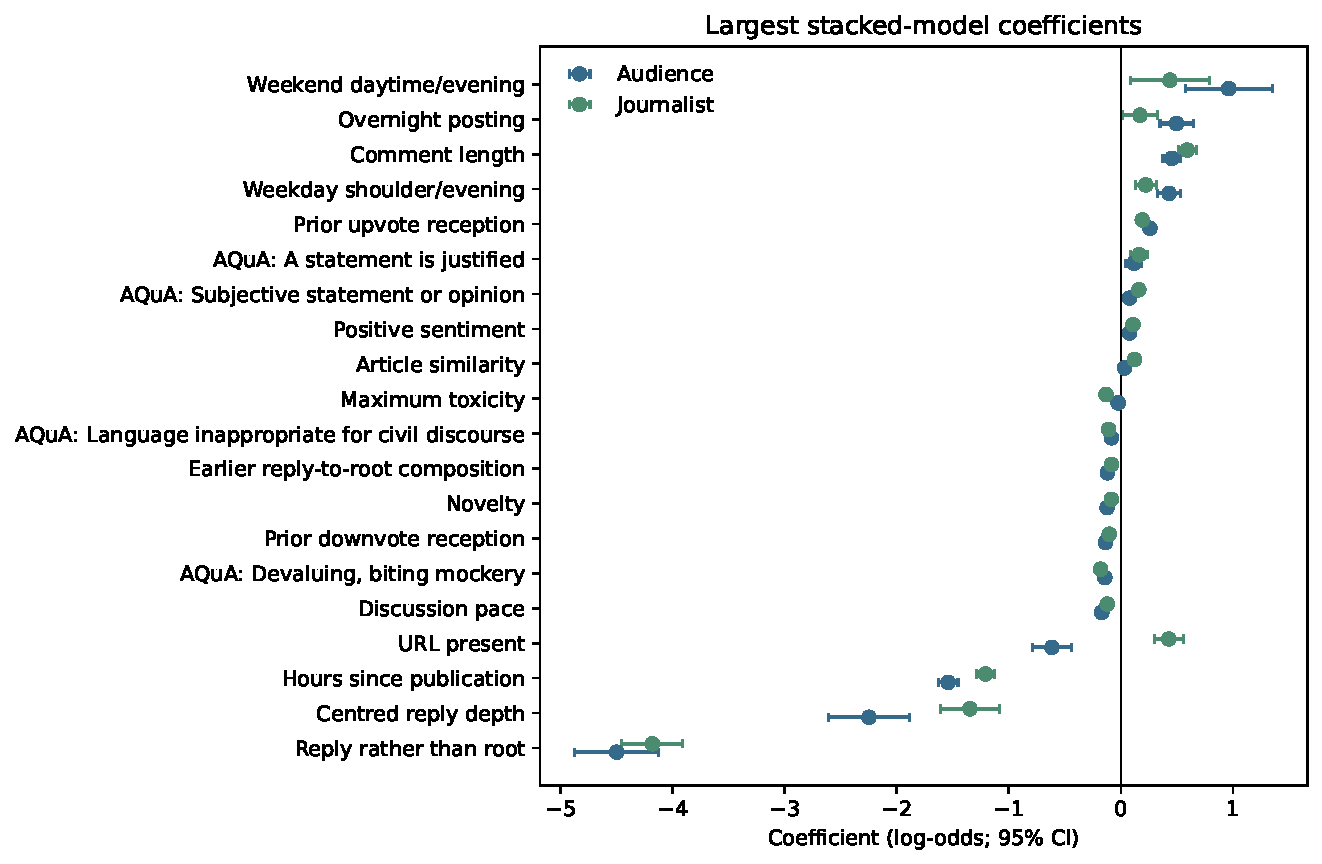
\includegraphics[width=\linewidth]{figures/regression_selector_coefficients.pdf}
\caption{Selector-specific conditional-logit for the largest absolute coefficients. Bars are 95\% article-clustered confidence intervals.}
\label{fig:selector-coefficients}
\end{figure}

Figure~\ref{fig:selector-differences} shows the largest feature coefficient differences between selectors. Relative to audiences, journalists have a stronger positive association with URL presence ($\Delta\beta=+1.044$, 95\% CI 0.892--1.196), and less negative associations with reply depth ($+0.901$, 0.519--1.282) and hours since publication ($+0.334$, 0.268--0.399). The coefficient for the author's earlier comments in the article is also more positive for journalists ($+0.123$, 0.058--0.187), although its journalist-specific association is close to zero ($\beta_J=+0.033$) and the audience association is negative ($\beta_A=-0.090$). URL presence is the clearest opposing-sign case: it is positive for journalists ($\beta_J=+0.428$) and negative for audiences ($\beta_A=-0.616$). Comment length is more positively associated with journalists ($\Delta\beta=+0.136$, 0.071--0.201), article similarity is also more positive ($+0.088$, 0.061--0.114), and toxicity is more negative ($-0.108$, $-0.127$ to $-0.090$). Audiences have relatively stronger associations with overnight posting ($\Delta\beta=-0.327$, $-0.451$ to $-0.204$), weekend daytime/evening ($-0.524$, $-0.809$ to $-0.239$), weekday shoulder/evening ($-0.207$, $-0.284$ to $-0.129$), and upvote reception in the author's prior comments ($-0.068$, $-0.086$ to $-0.050$). Journalist associations are relatively more positive for proposed solutions ($\Delta\beta=+0.098$, 0.059--0.137), relevance to the discussion ($+0.094$, 0.051--0.138), and subjective statements ($+0.083$, 0.046--0.120), whereas factual claims have the strongest negative gap ($-0.121$, $-0.189$ to $-0.052$). Personal stories are positively associated with both selectors but relatively more audience-associated ($\Delta\beta=-0.029$, $-0.054$ to $-0.004$). A positive difference means a more positive or less negative journalist vs audience association; it does not by itself mean that journalists positively select the feature.

\begin{figure}[t]
\centering
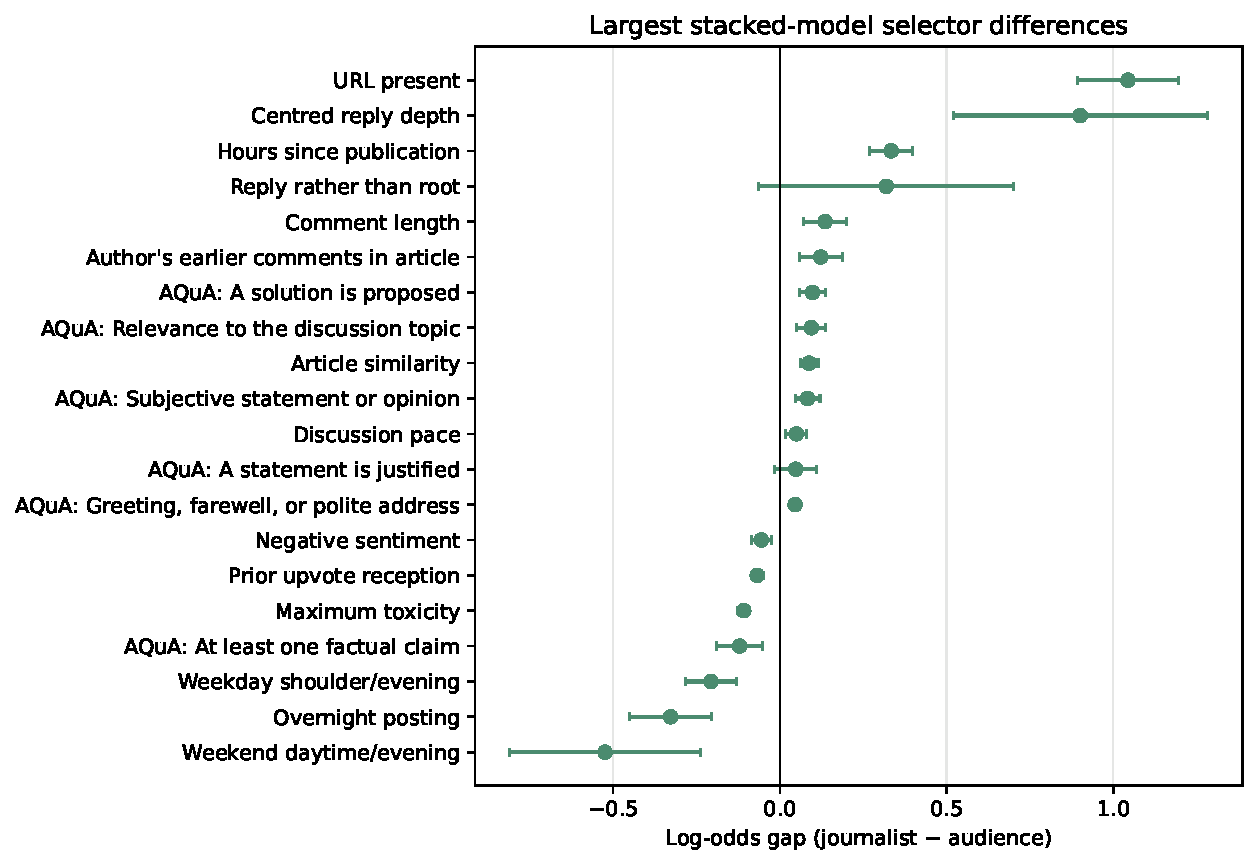
\includegraphics[width=\linewidth]{figures/regression_selector_differences.pdf}
\caption{Regression feature-level comment gaps for the twenty largest absolute differences, with 95\% article-clustered confidence intervals. Full estimates and diagnostics appear in Appendix~\ref{app:regression}.}
\label{fig:selector-differences}
\end{figure}

\subsubsection{Signed SHAP gaps}
The XGBoost attributions place timing and discussion structure among the largest signed contribution gaps (Figure~\ref{fig:xgb-shap}). For scalar-only XGB, the mean journalist-minus-audience contribution is $+0.1076$ for elapsed time, $+0.0780$ for discussion pace, and $-0.0717$ for reply status. With text embeddings, the corresponding gaps are $+0.0615$, $+0.0248$, and $-0.0463$. The signs persist within this family, although their magnitudes depend on each fitted model's score scale.

\begin{figure}[t]
\centering
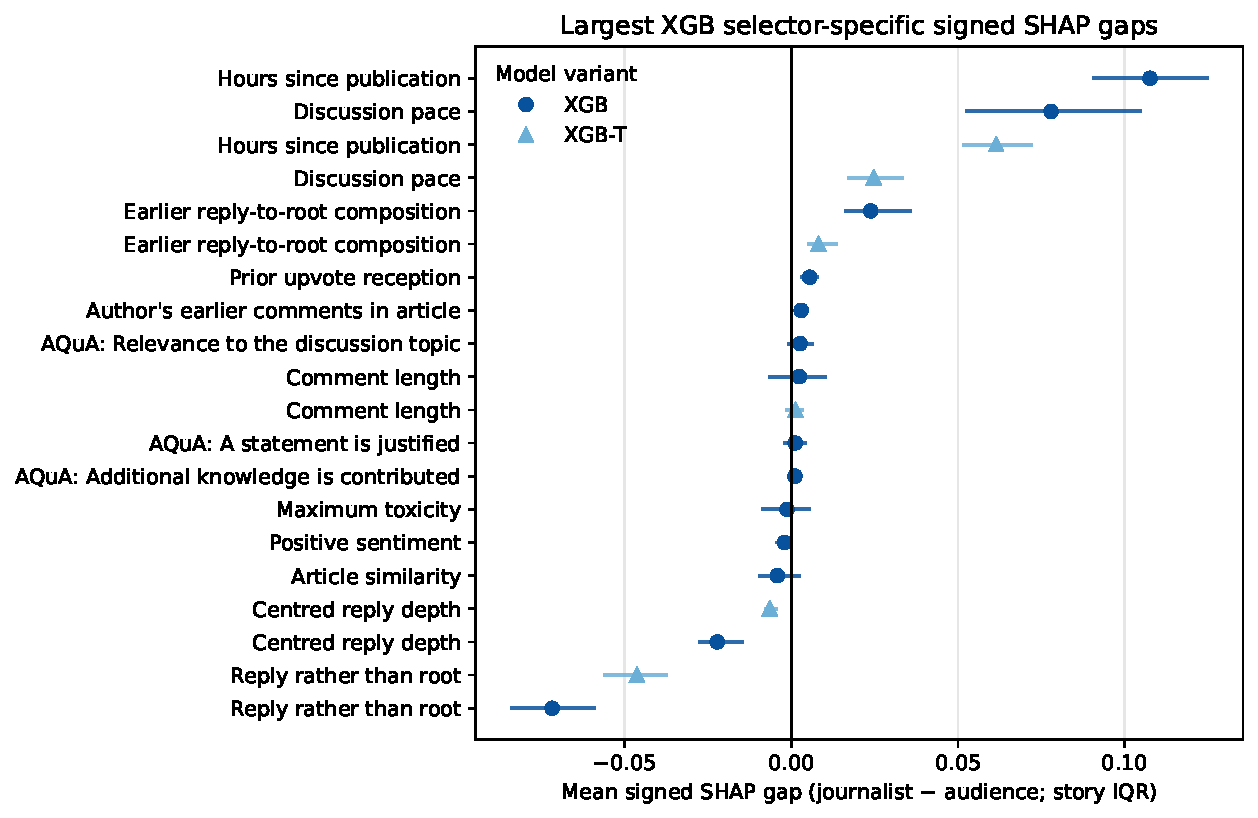
\includegraphics[width=\linewidth]{figures/xgb_signed_shap_gaps.pdf}
\caption{XGBoost signed SHAP gaps, bars show discussion-level interquartile ranges.}
\label{fig:xgb-shap}
\end{figure}

The neural models also assign a negative mean attribution gap to reply status: $-1.6322$ for NN and $-1.3588$ for NN-T (Figure~\ref{fig:nn-shap}). Discussion pace has positive gaps of $+0.0735$ and $+0.7291$, respectively. Earlier author participation has positive gaps ($+0.0978$ and $+0.0909$), whereas article similarity has negative gaps ($-0.0697$ and $-0.0809$). 

\begin{figure}[t]
\centering
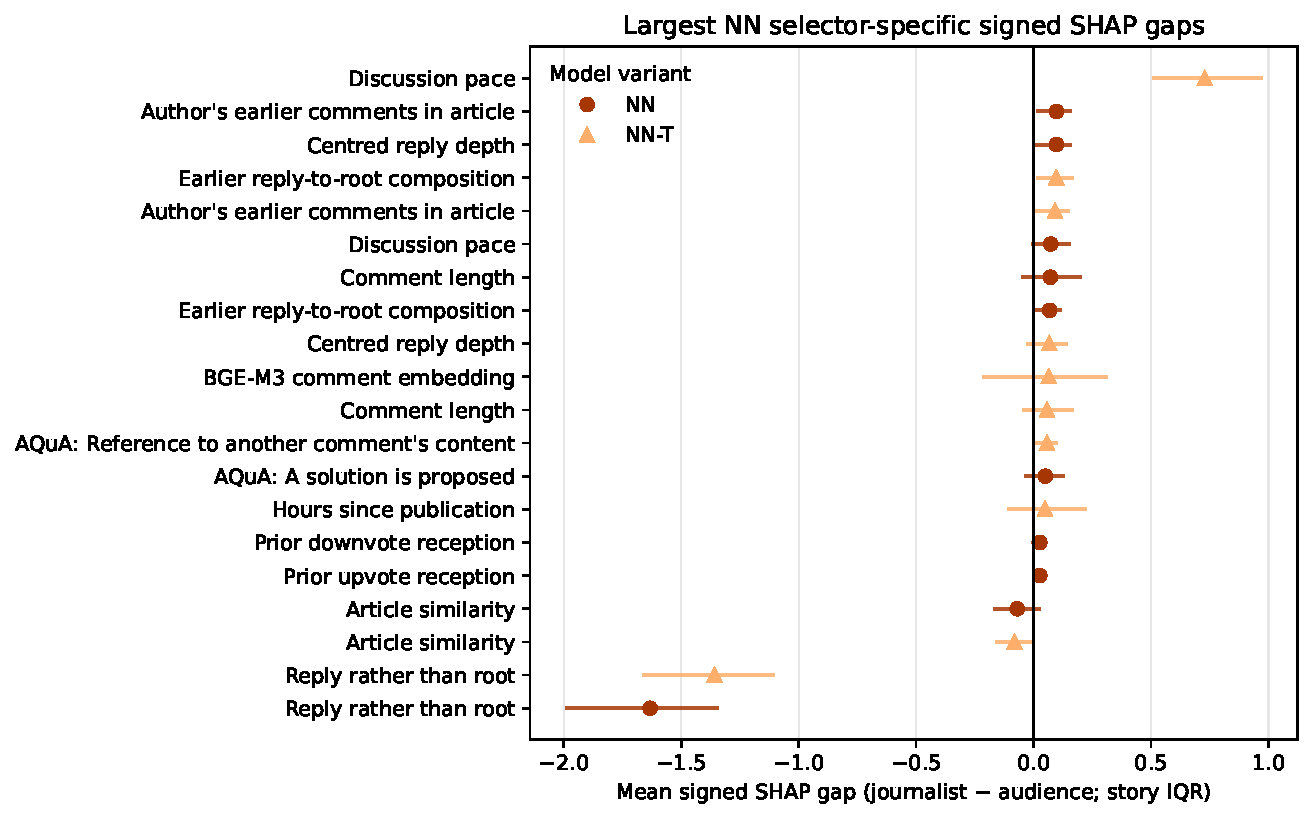
\includegraphics[width=\linewidth]{figures/nn_signed_shap_gaps.pdf}
\caption{Neural-network signed SHAP gaps, bars show discussion-level interquartile ranges.}
\label{fig:nn-shap}
\end{figure}

\subsubsection{Agreement and disagreement across feature-gap measures}
Figure~\ref{fig:regression-shap} compares all 41 scalar-feature regression gaps with each of the four ML variants. Some signs coincide: discussion pace has a positive regression gap ($+0.050$) and positive SHAP gaps in both ML families, and the author's earlier participation within the article has a positive regression gap ($+0.123$) and positive gaps in both neural variants. Other patterns depend on the model and estimand: reply depth has a positive regression gap and positive neural SHAP gaps ($+0.0970$ and $+0.0668$), but negative XGBoost gaps ($-0.0222$ and $-0.0064$). Article similarity has a positive regression gap but negative neural gaps. Signed SHAP summaries therefore do not consistently mirror the regression's journalist--audience coefficient differences. The fitted ML models offer a different descriptive account of feature contributions to selection scores. These contrasts are exploratory: coefficients describe conditional associations, whereas SHAP values describe contributions relative to a background prediction. Signed averages can also conceal offsetting contributions. Agreement or disagreement in sign consequently does not establish agreement or contradiction in the underlying selection associations.

\begin{figure}[t]
\centering
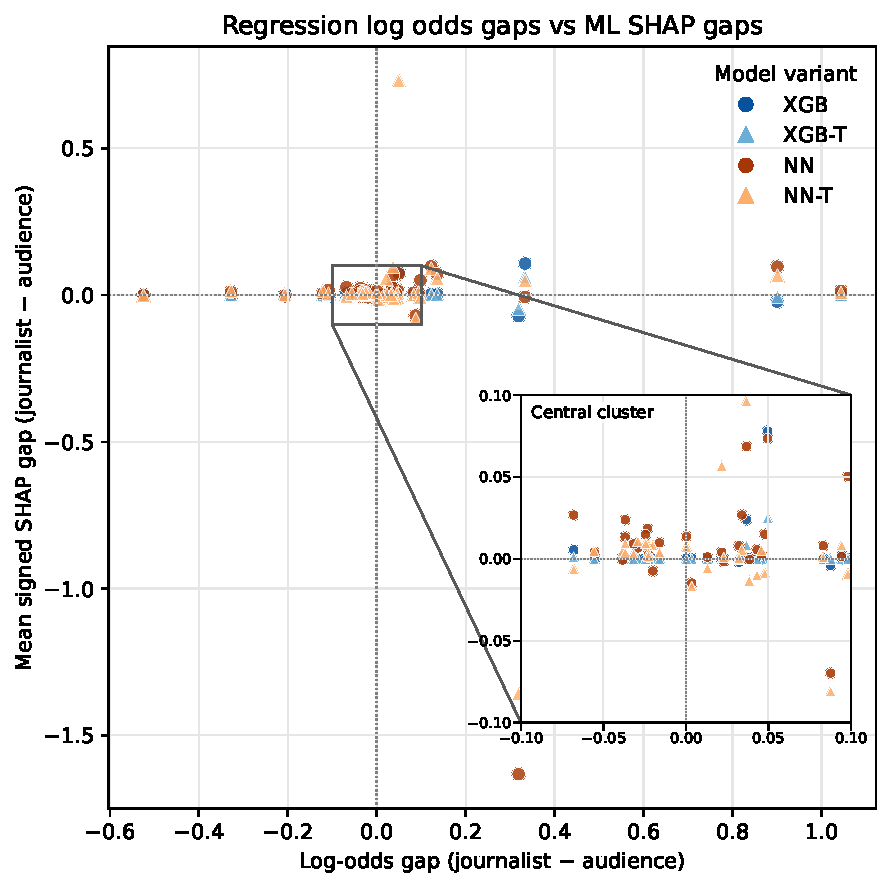
\includegraphics[width=\linewidth]{figures/regression_vs_shap_gaps.pdf}
\caption{Regression log-odds gaps versus ML signed SHAP gaps on 41 matched scalar-feature points.}
\label{fig:regression-shap}
\end{figure}

\subsection{Ranking model performance}
Table~\ref{tab:model-performance} reports the five fitted models and three fixed ranking baselines on the same 2,559 held-out discussions. XGBoost with text representations has the highest observed nDCG@$k$ for both editorial selection, 0.257 (95\% CI 0.247--0.267), and audience selection, 0.240 (0.231--0.250). Adding text representations increases the nDCG point estimate for each ML family and selector (significant at 95\% confidence for all except the neural audience selector). All scores remain far below 1.0, reflecting the difficulty of full-discussion retrieval for small n.

\begin{table*}[t]
\centering
\small
\begin{tabular}{lllll}
\toprule
Model & Audience nDCG@k & Editor nDCG@k & Audience macro-F1 & Editor macro-F1 \\
\midrule
Reg & 0.232 [0.222, 0.241] & 0.232 [0.222, 0.241] & 0.892 [0.889, 0.896] & 0.892 [0.889, 0.895] \\
XGB & 0.232 [0.222, 0.242] & 0.246 [0.236, 0.256] & 0.887 [0.884, 0.891] & 0.893 [0.890, 0.896] \\
XGB-T & \textbf{0.240 [0.231, 0.250]} & \textbf{0.257 [0.247, 0.267]} & 0.887 [0.884, 0.890] & \textbf{0.894 [0.891, 0.897]} \\
NN & 0.222 [0.212, 0.231] & 0.226 [0.217, 0.236] & \textbf{0.892 [0.889, 0.895]} & 0.892 [0.889, 0.895] \\
NN-T & 0.225 [0.216, 0.235] & 0.244 [0.234, 0.253] & 0.887 [0.883, 0.890] & 0.892 [0.889, 0.894] \\
\midrule
Earliest & 0.147 [0.139, 0.155] & 0.112 [0.105, 0.120] & 0.818 [0.814, 0.822] & 0.780 [0.774, 0.785] \\
Roots/earliest & 0.157 [0.148, 0.165] & 0.121 [0.114, 0.129] & 0.875 [0.872, 0.879] & 0.870 [0.867, 0.874] \\
Longest & 0.033 [0.029, 0.038] & 0.042 [0.037, 0.046] & 0.638 [0.633, 0.643] & 0.677 [0.672, 0.682] \\
\bottomrule
\end{tabular}

\caption{Held-out model performance, with 95\% article-bootstrap intervals. Macro-F1 uses balanced selected/non-selected subsamples; nDCG uses complete discussions. Baselines order by earliest posting (Earliest), roots before replies and then earliest posting (Roots/earliest), or descending word count (Longest); ties use comment ID.}
\label{tab:model-performance}
\end{table*}

Balanced-sample macro-F1 lies between 0.887 and 0.894 across the held-out fitted-model--selector combinations. Its high level reflects the distinct (easier) balanced comparison task and does not mean that models recover almost nine in ten selections from full discussions. For contextual comparison, He et al.~\citep{He2024} report global macro-F1 around 0.75 in their New York Times setting.

\subsubsection{Model-implied comment gap}
The model-implied gap compares the top-$k$ comments produced by the journalist score with the ranking produced by the audience score of a particular model. On held-out discussions, the equal-discussion mean normalised rank gaps are $0.0063$ for regression, $0.0010$ for XGB, $0.0003$ for XGB-T, $0.0088$ for NN, and $0.0177$ for NN-T. All are far below the random-set expectation of $0.5$ and below the observed gap of $0.0725$. Replacing the observed sets in the Jaccard calculation with each model's two fitted top-$k_j$ sets gives mean model-implied Jaccard gaps of $0.4272$ for regression, $0.1344$ for XGB, $0.0588$ for XGB-T, $0.4411$ for NN, and $0.5473$ for NN-T. The fitted models therefore recover similar ranking patterns for journalists and the audience. However, small normalised rank gaps do not lead to strong agreement on top-set membership. Shared representations in the ML models are a possible explanation for their similar rankings, but this mechanism is not isolated by the present comparison.

\section{Discussion}
We examined how editorial curation and audience endorsement converge and diverge across 5,118 news discussions. For RQ1, journalists' selections generally rank highly with readers: the mean normalised rank gap is 7.25\%, compared with 50\% for random selection. Yet mean Jaccard similarity is 58.79\%, showing that broad agreement about which comments deserve attention can coexist with differences in the small set chosen for prominence. This extends the news-gap perspective from the choice of news stories to the recognition of readers' contributions within them.

For feature-level RQ2 analysis, journalists and readers both select longer, earlier, less toxic comments and favour root comments over replies, conditional on the other measured characteristics. Their differences are more specific than a simple contrast between professional quality and popular appeal. Journalists have stronger positive associations with length and article similarity, a positive association with links where readers have a negative one, and a stronger negative association with toxicity. Readers' selections are more strongly associated with factual claims, previous audience approval of the author, and posting outside weekday working hours. A factual-claim score indicates that a claim is made, not that it is true. Similarly, a link is not evidence that its source is reliable. The editorial association with proposed solutions nevertheless suggests that constructive contributions can receive recognition beyond what audience votes alone would identify. The weaker negative editorial associations with reply depth and delay also suggest that these features differentiate curation from audience endorsement, without implying that editors favour deep replies or late comments in absolute terms.

Our editorial associations with length, article relevance, positive sentiment, and lower toxicity are consistent with the characteristics of English language New York Times editor-picks reported by \citet{He2024}. We extend this comparison by distinguishing characteristics associated with editorial selection from those that distinguish editors from readers. The comparison matters because a characteristic of Editors' Picks need not be uniquely editorial. Differences across platforms may reflect community norms, available voting mechanisms, and the visibility given to curated comments, as well as different editorial selection priorities.

Timing and discussion structure also suggest that recognition depends on opportunities to be seen. Early root comments can reach readers before a discussion becomes crowded, while replies may address a smaller group already involved in an exchange. Editors' Picks receive additional prominence, creating the possibility that editorial attention generates audience endorsement as well as responding to it. We cannot separate these mechanisms using our snapshot. Newsrooms seeking to recognise a wider range of contributors could examine whether worthwhile late comments and exchanges within reply threads are being overlooked, rather than interpreting low votes as evidence of low value.

For RQ3, the predictive models offer a possible way to help editors shortlist candidate contributions in discussions with hundreds of comments, or help readers find high quality comments that have not received attention. Text-enabled XGBoost has the highest observed held-out nDCG (0.257 for editorial and 0.240 for audience selection), but retrieval remains imperfect. The models do not establish an acceptable error rate for deployment, and the high balanced-sample F1 scores should not be interpreted as near-complete recovery of selections in a live forum.

Finally, the smaller model-implied gaps suggest that the models reproduce shared ranking patterns more readily than the particular choices that distinguish journalists and readers. Disagreement between regression and SHAP summaries limits a single feature-based explanation of these choices: conditional slopes and average contributions to nonlinear scores answer different questions. Shared rankings may reflect shared evaluative priorities, shared exposure, or both. For news organisations, votes and editorial choices are therefore useful complementary indicators, whose meaning depends on whether a discussion is intended to surface curated information or support exchange among readers.

\section{Limitations and Ethical Considerations}
\label{sec:ethics}
The study extends evidence beyond English-language and oft-studied New York Times settings, but still concerns a single German-language news forum and a selected population of commenters and voters. Editors' Picks are sparse institutional actions, and the people making these professional selections may vote differently in a personal capacity---though we emphasise that we are explicitly studying this professional vs (audience) personal gap. Deletion also limits the available evidence. Across the full collection, 193,090 of 9,415,942 retrieved records (2.05\%) were deletion markers without comment content. Missing contributions may differ systematically from those retained.

Retrospective vote counts and pinned status limit temporal interpretation. Votes and pinning can, and likely do, influence one another through exposure, potentially contributing to the apparent agreement between selectors. This means our comment gap of 7.25\% is likely a lower bound on the true gap between independent editorial and audience preferences. Default and alternative comment orders also affect what readers encounter. Future work could collect repeated snapshots as discussions unfold or partner with newsrooms to obtain timestamped votes, pinning decisions, moderation events, and impression data. This would help distinguish characteristics associated with selection from the visibility that precedes or follows it.

Automated language measures introduce further uncertainty. Research on English-language hate-speech detection documents dialect-related bias \citep{Sap2019} and misleading associations with identity terms \citep{Kennedy2020}. Sarcasm, dialect, short replies, and arguments that depend on surrounding discussion warrant particular attention rather than an assumption that an off-the-shelf score always transfers reliably to this forum. Future work should validate these scores against independently annotated comments.

The study received institutional ethics review approval (ID 13838441). The project follows the Association of Internet Researchers' ethics framework \citep{AoIR2019} and, whilst it is not feasible or methodologically prudent to seek informed consent at scale, considers contextual privacy and potential harm throughout the research process. Data collection followed the site's robots.txt directives and terms \citep{DerStandard2024, DerStandardRobots2026}. The collector retrieved public records without posting comments, voting, or otherwise participating in discussions. Author identifiers were replaced by keyed hashed pseudonyms during collection. This enables longitudinal linkage but does not anonymise the data: verbatim text, timestamps, and histories may remain identifying or searchable. We share code, documentation, and aggregate results while withholding the full comment-level dataset to reduce risks to commenters' privacy.

Uncritical application of our findings could reinforce the visibility of already prominent contributors or dominant viewpoints if observed selections are treated as an objective quality standard. False promotions could elevate unsuitable contributions, while omissions could deny useful contributions attention. The models could also be misused to profile authors, automate suppression, or optimise comments to game editorial and voting signals.

\section{Conclusion}
Using 2.39 million comments across 5,118 \textit{Der Standard} articles published in 2025, we quantified agreement between editorial selections and audience votes, compared their associated comment characteristics, and evaluated models for recovering these selections. The mean normalised rank gap of 7.25\% indicates that Editors' Picks generally occupy high audience ranks---this corresponds illustratively to a mean rank of about 36.2 out of 467.6 comments. Mean Jaccard similarity of 58.79\% however shows that the selected small sets remain somewhat distinct. Journalists have stronger associations with length and article similarity, favour links relative to readers, and have a stronger negative association with toxicity. Audience selection is more strongly associated with factual claims, authors' previous audience approval, and posting outside weekday working hours. These are conditional associations, and several feature-gap directions differ across regression and nonlinear attribution summaries.

Text-enabled XGBoost achieves held-out nDCG@$k$ of 0.257 for editorial and 0.240 for audience selection, with balanced-sample macro-F1 of 0.894 and 0.887. Recovering a few selected contributions from hundreds of comments remains difficult, particularly when the timing of exposure and selection is unobserved. Model-implied rank gaps of 0.03--1.77\% suggest that the fitted models capture shared ranking patterns more readily than selector-specific choices. Nevertheless, the models could help editors find candidate pick contributions in large discussions or help readers find high-quality comments that have not received attention.

News comments give readers a way to contribute knowledge, experience, and criticism to journalism. Understanding which contributions receive recognition can help newsrooms make better use of this participation while attending to readers whose contributions attract less visibility.

\section*{Acknowledgments}
OpenAI Codex was used in co-writing analysis code and reorganising author-written manuscript text.
